\documentclass[11pt]{amsart}
\usepackage{amsmath}
\usepackage{geometry}                % See geometry.pdf to learn the layout options. There are lots.
\geometry{letterpaper}                   % ... or a4paper or a5paper or ... 
%\geometry{landscape}                % Activate for for rotated page geometry
%\usepackage[parfill]{parskip}    % Activate to begin paragraphs with an empty line rather than an indent
\usepackage{graphicx}
\usepackage{caption}
\usepackage{subcaption}
\usepackage{amssymb}
\usepackage{epstopdf}
\usepackage[]{algorithm2e}

\title{COMP 652: Assignment 2}
\author{Carlos G. Oliver (ID: 260425853)}
\date{\today}                                           % Activate to display a given date or no date


\newcommand\independent{\protect\mathpalette{\protect\independenT}{\perp}}
\DeclareMathOperator{\E}{\mathbb{E}}
\def\independenT#1#2{\mathrel{\rlap{$#1#2$}\mkern2mu{#1#2}}}
\newcommand{\vek}[1]{\mathbf{#1}}

\begin{document}
\maketitle
\section{Q1: Properties of entropy and mutual information, and Bayes net construction}
\subsection{(a)} Prove that $H(X) \geq H(X \vert Y)$, with equality achieved when $X$ and $Y$ are independent.

\begin{proof}

We begin with the following relation:

\begin{equation}
H(X) = H(X \vert Y) + I(X ; Y)
\end{equation}

Where $I(X;Y)$ is the mutual information between the two random variables $X$ and $Y$. This quantity represents the amount of information that can be obtained about one random variable, knowing the other. We can arrive at the above equation from the formal definition of mutual information:

\begin{equation}
\begin{aligned}
I(X;Y) & = \sum_{x,y}p(x,y) \log\bigg(\frac{p(x,y)}{p(x)p(y)}\bigg) \\
	& = \sum_{x,y}p(x,y) \bigg[\log \bigg(\frac{p(x,y)}{p(y)} \bigg) - \log p(x) \bigg] \\
	& = \sum_{x,y}p(x, y) \log\bigg(\frac{p(x,y)}{p(y)}\bigg) - \sum_{x,y}p(x, y) \log p(x) \\
	& = \sum_{x,y}p(y) p(x \vert y) \log p(x \vert y) - \sum_{x,y}p(x, y) \log p(x) && \text{using:}  p(x,y) = p(x \vert y)p(y) = p(y \vert x) p(x) \\
	& = \sum_{y} p(y) \sum_{x} p(x \vert y) - \sum_{x} \log p(x) \sum_{y} p(x,y) && \text{breaking up summations} \\
	&= - \sum_{y} p(y) H(X \vert Y=y) - \sum_{x} \log p(x) \sum_{y} p(x,y) && \text{by definition of entropy} \\
	&= - H(X \vert Y) - \sum_{x}p(x) \log p(x) && \text{marginal probability} \\
	&= - H(X \vert Y) - H(X) \\
	&= H(X) - H(X \vert Y)
\end{aligned}
\label{eq:mutual}
\end{equation}

In order to prove the original statement, it suffices to show that $I(X;Y) \geq 0$ with equality when  $X \independent Y$.

We need a few definitions in order to show this. First, we define the KL-divergence between two probability distributions $P$ and $Q$ as:

\begin{equation}
D_{KL} = \sum_{x} P(x) \log \frac{P(x)}{Q(x)}
\end{equation}

Which is related to the mutual information of two random variables $X$ and $Y$ as:

\begin{equation}
I(X;Y) = D_{KL}\big(P(X,Y) \vert \vert P(X)P(Y)\big) = \sum_{x,y} p(x,y) \log \bigg( \frac{p(x,y)}{p(x)p(y)} \bigg)
\label{eq:kl-mutual}
\end{equation}

We will use Jensen's inequality which applies to the expected value of convex functions of random variables, such that if $f(x)$ is a convex function, then $\E [f(x)] \geq f(\E [x]))$. By letting the negative logarithm be the convex function, we can show that $I(X;Y) \geq 0$.

\begin{equation}
\begin{aligned}
-\sum_{x,y} p(x,y) \log(\frac{p(x)p(y)}{p(x,y)} & \geq -\log \bigg( \sum_{x,y} p(x,y) \frac{p(x)p(y)}{p(x,y)} \bigg) \\
								   & \geq -\log \bigg ( \sum_{x,y} p(x)p(y) \bigg) \\
								   & \geq -\log \bigg( \sum_{x} p(x) \sum_{y} p(y) \bigg) \\
								   & = 0 && \text{probabilities sum to 1}
\label{eq:mutual-pos}
\end{aligned}
\end{equation}

It is easy to see that for the case where $X \independent Y$ we have $p(x,y) = p(x)p(y)$ so 

\begin{equation}
\sum_{x,y} p(x,y) \log\bigg(\frac{p(x,y)}{p(x)p(y)}\bigg) = \sum_{x,y} p(x,y) \log\bigg(\frac{p(x)p(y)}{p(x)p(y)}\bigg) = 0
\end{equation}

\end{proof}


\subsection{(b)}

Given the relation between KL divergence and mutual information in Equation ~\ref{eq:kl-mutual} we showed in Equation ~\ref{eq:mutual-pos} that this quantity is $D_{KL} \geq 0$. 

The KL divergence is not a symmetric quantity. Let $P(x) = 1$ for all values of $x$ and let $Q(x) = 0	$ for all values of x. 

\begin{equation}
D_{KL}(P, Q) = \sum_{x}0 \log \frac{0}{1} = 0
\end{equation}

\begin{equation}
D_{KL}(Q,P) = \sum_{x}1 \log \frac{1}{0} = \infty
\end{equation}


\subsection{(c)}

Show that $I(X;Y) = H(X) + H(Y) - H(X,Y)$, also known as the chain rule for conditional entropy.

\begin{proof}

We first show that $H(X \vert Y) = H(X,Y) - H(X)$.

\begin{equation}
\begin{aligned}
H(X\vert Y) &= \sum_{x,y}p(x,y) \log \bigg( \frac{p(y)}{p(x,y)} \bigg) \\
		 &= \sum_{x,y} p(x,y) \bigg[\log p(y) - \log p(x,y) \bigg] \\
		 &= -\sum_{x,y}p(x,y) \log p(x,y) + \sum_{x,y} p(x,y) \log p(y) \\
		 &= H(X,Y) + \sum_{x,y} p(x,y) \log p(y) && \text{definition of entropy}\\
		 &= -H(X,Y) - H(X) 				      &&\text{marginalize out x as before}
\end{aligned}
\end{equation}

From this we obtain the expression $H(X,Y) = H(X) - H(X \vert Y)$ and substitute it into the statement to prove.

\begin{equation}
\begin{aligned}
I(X;Y) = H(X) + H(Y) - H(X,Y) = H(Y) - H(X \vert Y)
\end{aligned}
\end{equation}

Which we proved from the definition of $I(X;Y)$ in Equation ~\ref{eq:mutual} above.

\end{proof}

\subsection{(d)}

Shown in Equation ~\ref{eq:mutual-pos}


\subsection{(e)}

Let $\mathcal{X}_{i}$ represent the possible values of the random variable $x_i$ and $\mathcal{X}_{\pi_{i}}$ represent the possible values of the set of parents $x_{\pi_{i}}$.

\begin{equation}
\begin{aligned}
L(G \vert D) & = \prod_{j=1}^m p(\vek{x_j} \vert G) && \text{by definition of likelihood} \\
		   & = \prod_{j=1}^m \prod_{i=1}^n p(\vek{x_{j,i}} \vert G) && \text{by graph factorization} \\
		   & = \sum_{j=1}^{m}\sum_{i=1}^n \log p(x_{j,i} \vert G) \\
		   & = \sum_{j=1}^{m}\sum_{i=1}^n \log p(x_{j,i} \vert x_{\pi_{i}}) \\
		   & = \sum_{i=1}^{n}\sum_{j=1}^m \log p(x_{j,i} \vert x_{\pi_{i}}) && \text{sum over $m$ produces empirical distribution} \\
		   & = \sum_{i=1}^{n} \bigg[ \sum_{\mathcal{X}_{i}} \sum_{\mathcal{X}_{\pi_i}} N(x_{i}, x_{\pi_i}) \log (\hat{p} (x_{i} \vert x_{\pi_i}))\bigg] \\
		   &=  m \sum_{i=1}^{n} \bigg[ \sum_{\mathcal{X}_{i}} \sum_{\mathcal{X}_{\pi_i}} \frac{N(x_{i}, x_{\pi_i})}{m} \log (\hat{p} (x_{i} \vert x_{\pi_i}))\bigg]  && \text{multiply by $\frac{m}{m}$}\\	
		   &=  m \sum_{i=1}^{n} \bigg[ \sum_{\mathcal{X}_{i}} \sum_{\mathcal{X}_{\pi_i}} \frac{N(x_{i}, x_{\pi_i})}{m} \log \frac{\hat{p} (x_{i}, x_{\pi_i})}{\hat{p}(x_{\pi_i})}\bigg]  && \text{definition of empirircal dist.} \\
		   &=  m \sum_{i=1}^{n} \bigg[ \sum_{\mathcal{X}_{i}} \sum_{\mathcal{X}_{\pi_i}} \frac{N(x_{i}, x_{\pi_i})}{m} \log \frac{\hat{p} (x_{i}, x_{\pi_i})}{\hat{p}(x_{\pi_i})} \frac{\hat{p}(x_{i})}{\hat{p}(x_{i})}\bigg]  && \text{}  \\
		   &=  m \sum_{i=1}^{n} \bigg[ \sum_{\mathcal{X}_{i}} \sum_{\mathcal{X}_{\pi_i}} \hat{p}(x_i, x_{\pi_i}) \log \frac{\hat{p} (x_{i}, x_{\pi_i})}{\hat{p}(x_{\pi_i})} \frac{\hat{p}(x_{i})}{\hat{p}(x_{i})}\bigg]  && \text{frequencies of joint divided by $m$ is joint.}   \\
		   &=  m \sum_{i=1}^{n} \bigg[ \sum_{\mathcal{X}_{i}} \sum_{\mathcal{X}_{\pi_i}} \hat{p}(x_i, x_{\pi_i}) \bigg\{ \log \frac{\hat{p} (x_{i}, x_{\pi_i})}{\hat{p}(x_{\pi_i}) \hat{p}(x_{i})} + \log {\hat{p}(x_{i})} \bigg\} \bigg] && \text{break up log of products} \\
		   &= m \sum_{i=1}^n MI_{\hat{p}}(X_i, X_{\pi_i}) - m \sum_{i=1}^n H_{\hat{p}}(X_i)  && \text{by definition of mutual info. and entropy}
\end{aligned}
\label{eq:graph-likelihood}
\end{equation}

\subsection{(f)}

If graphs $G_1$ and $G_2$ are identical except for one extra arc in $G_2$ we consider the node with an extra incoming arc in $G_2$ whose set of parents is now $x_{\pi_i \cup \tilde{x}}$ Using the equation for the likelihood of a graph derived in Eq. ~\ref{eq:graph-likelihood} we see that the second term depends only on the entropy of each node and not on the parents these quantities will not change. The mutual information term only depends on the node being considered and its set of parents $X_{\pi_i}$ therefore all other terms in the sum remain equal and we can only consider the node $X_i$ in $G_1$ and $G_2$ where the additional arc was inserted.

We use an expansion of mutual information between a node and its parents derived in ~\cite{campos2006scoring} where $\vert X_{\pi_i} \vert = L$:

\begin{equation}
MI_{\hat{P}}(X_i, X_{\pi_i}) = MI_{\hat{P}}(X_i, X_{\pi_{i}}^{1}) + \sum_{l = 2}^{L} MI_{\hat{P}}(X_i, X_{\pi_i}^{l} \vert \{X_{\pi_i}^{1},..., X_{\pi_i}^{L-1}\})
\end{equation}

Using the same expansion we can compute the mutual information at the node with extra parent $\tilde{X}$ and so $\vert X_{\pi_i} \cup \tilde{X} \vert = L + 1$

\begin{equation}
\begin{aligned}
MI_{\hat{P}}(X_i, X_{\pi_i} \cup \tilde{X}) &= MI_{\hat{P}}(X_i, \tilde{X}) + \sum_{l = 2}^{L+1} MI_{\hat{P}}(X_i, X_{\pi_i}^{l} \vert \{X_{\pi_i}^{1},..., X_{\pi_i}^{L-1}\}) \\
								  &= MI_{\hat{P}}(X_i, \tilde{X}) + MI_{\hat{P}}(X_i, X_{\pi_{i}}^{1}) + \sum_{l = 3}^{L+1} MI_{\hat{P}}(X_i, X_{\pi_i}^{l} \vert \{X_{\pi_i}^{1},..., X_{\pi_i}^{L-1}\})
\end{aligned}
\end{equation}

\begin{proof}
\begin{equation}
\begin{aligned}
MI_{\hat{p}}(X_i, X_{\pi_i}) &<  MI_{\hat{p}}(X_i, X_{\pi_i \cup \tilde{X}}) \\
MI_{\hat{P}}(X_i, X_{\pi_{i}}^{1}) + \sum_{l = 2}^{L} MI_{\hat{P}}(X_i, X_{\pi_i}^{l} \vert \{X_{\pi_i}^{1},..., X_{\pi_i}^{L-1}\}) &< MI_{\hat{P}}(X_i, \tilde{X}) +\\ 
& MI_{\hat{P}}(X_i, X_{\pi_{i}}^{1}) + \sum_{l = 3}^{L+1} MI_{\hat{P}}(X_i, X_{\pi_i}^{l} \vert \{X_{\pi_i}^{1},..., X_{\pi_i}^{L-1}\}) \\
0 &< MI_{\hat{p}}(X_i, \tilde{X})
\end{aligned}
\end{equation}


\end{proof}

\section{Q2: Sigmoid Bayes nets}

Since by construction, bayes nets are DAGs and nodes are separated into two layers, we assume the architecture illustrated in {\bf Fig ~\ref{fig:bayes}}.

\begin{figure}
\centering
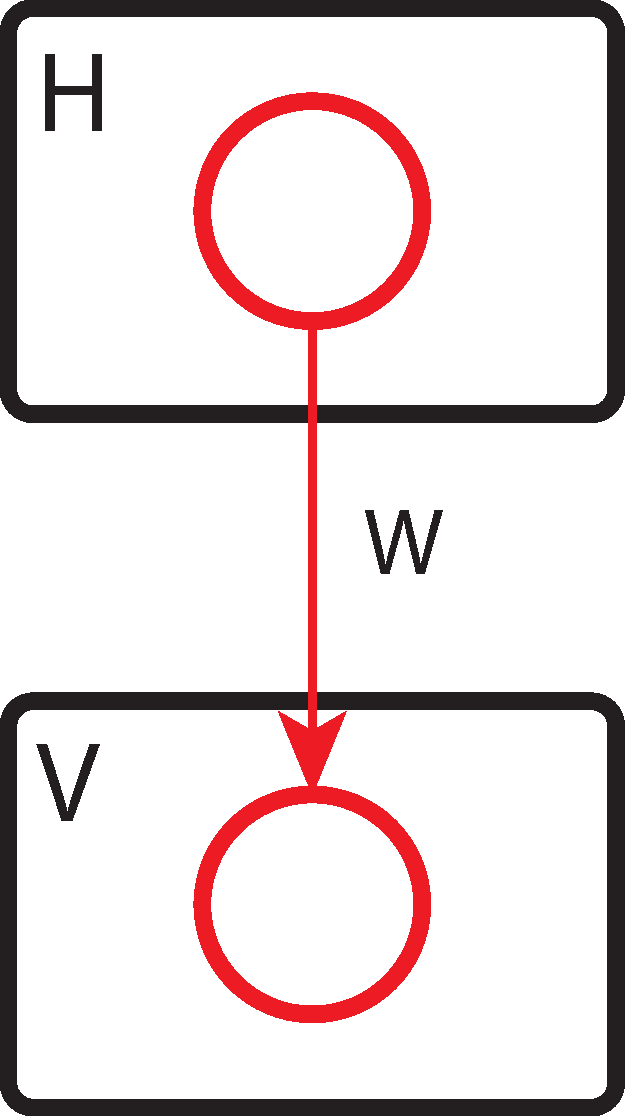
\includegraphics[height=0.2\textheight]{Figures/bayes.pdf}
\caption{Bayes net with one hidden layer parametrized by weight matrix $W$.}
\label{fig:bayes}
\end{figure}

We want to find the $W$ that maximizes the likelihood that the hidden nodes $H$ generated the data seen by the visible nodes $V$. Let us assume we receive a set of values $D$ for the visible nodes which we represent as the vector $\vek{v}$. We wish to maximize the likelihood over all data vectors in $D$ with respect to the weight of each connection $w_{ij}$.

In the following derivation (based on the text by Neal Radford ~\cite{neal1992connectionist}), we will be making use of Bayes rule on the probability of the vector $\vek{x}$ of nodes in graph $X$ which can be viewed as the joint probability over all nodes in the graph, given the values of the visible nodes. Note that we can form the vector of nodes $x$ by joining the vectors of visible and hidden nodes as $\vek{x} = \langle \vek{v}, \vek{h} \rangle$.

\begin{equation}
P(X= \langle \vek{v}, \vek{h} \rangle) = P(X = \langle \vek{v}, \vek{h} \rangle \vert V = \vek{v}) P(V = \vek{v})
\end{equation}

Now we maximize the log likelihood of the data with respect to the weights.

\begin{equation}
\begin{aligned}
\frac{\partial L}{\partial w_{ij}} &= \frac{\partial}{\partial w_{ij}} \log \prod_{\vek{v} \in D} P(V = \vek{v}) \\
						 & =  \frac{\partial}{\partial w_{ij}} \sum_{\vek{v} \in D} \log P(V = \vek{v}) \\
						 & =  \sum_{\vek{v} \in D}  \frac{1}{P(V = \vek{v})} \frac{\partial}{\partial w_{ij}} P(V = \vek{d}) \\
						 & =  \sum_{\vek{v} \in D}  \frac{P(X = \vek{x} \vert V = \vek{v})}{P(X = \vek{x})} \frac{\partial}{\partial w_{ij}} P(V = \vek{d}) && \text{bayes rule}\\
						 & = \sum_{\vek{v} \in D}  \frac{P(X = \langle \vek{v}, \vek{h} \rangle \vert V = \vek{v})}{P(X = \langle \vek{v}, \vek{h} \rangle)}  \sum_{h \in H} \frac{\partial}{\partial w_{ij}} P(X=\langle \vek{v}, \vek{h} \rangle) && \text{marginalizing over H} \\
						 & = \sum_{\vek{v} \in D}   \sum_{\vek{x}} \frac{P(X = \vek{x}  \vert V = \vek{v})}{P(X = \vek{x)}}  \frac{\partial}{\partial w_{ij}} P(X=\vek{x}) && \text{use given parametrization} \\
						 & = \sum_{\vek{v} \in D}   \sum_{\vek{x}} P(X = \vek{x}  \vert V = \vek{v}) \frac{1}{\sigma(X_i \sum_{j \in \pi_i} w_{ij}X_j)} \frac{\partial}{\partial w_{ij}} \sigma(X_i \sum_{j \in \pi_i} w_{ij}X_j)) && \text{multiply by $X_i$ for binary values} \\
						 & = \sum_{\vek{v} \in D}   \sum_{\vek{x}} P(X = \vek{x}  \vert V = \vek{v}) X_{i} X_{j} \sigma(-X_{i} \sum_{\pi_i} w_{ij} X_{j})
\end{aligned}
\end{equation}

From this we can get an update rule for $w_{ij}$ as:

\begin{equation}
w_{ij}^{new} = w_{ij} + \alpha X_{i} X_{j} \sigma(-X_{i} \sum_{\pi_i} w_{ij} X_{j})
\end{equation}

We can generate samples for $P(X = \vek{x}  \vert V = \vek{v})$ using Gibbs sampling, by fixing the visible nodes to a certain value and sampling for the hidden nodes. 


\bibliographystyle{plain}
\bibliography{A2_cgo}

\end{document}  